%!TEX root = main.tex

\chapter{Basic Syntax and Semantics}

We are now ready to discuss the predicate logic, mostly the first-order logic. The language of predicate logic is more expressive than the one of propositional logic and allows us to express complex formulas in a much more concise way. In propositional logic, we often needed to use many variables and created long formulas. In predicate logic, some of these can be written more elegantly, as we can now use functions, relations, and logical quantifiers.

This whole part will follow the structure of the previous one -- we will again start by the basic syntax and semantics of predicate logic, then we will discuss the logical theories and their models, the tableau method in predicate logic and also the resolution method. While the basic ideas remain the same, there are also important differences. For example, a model of a theory will now be defined as a mathematical structure in which all the axioms of the theory are true, instead of the simpler definition as a truth assignment.

\section{First-order formulas and theories}

The symbols used in first-order language can be divided into two groups -- symbols of logic and non-logical symbols. The \emph{symbols of logic} consist of \emph{variables} ($x, y, z, \dots, x_1, x_2, \dots \in \SVar$), logical connectives $(\to, \land, \lor, \lequiv, \neg)$, the quantifiers $(\forall x), (\exists x)$ for each variable $x \in \SVar$, and parenthesis. 

The \emph{non-logical symbols} consist of function symbols $(f, g, \dots)$, including constant symbols ($c, d, \dots$), which are nullary function symbols, and relation (predicate) symbols $(P, Q, R)$. Each function and relation symbol $S$, has an associated arity $\ar(S)\in\Nat$ that expresses the number of arguments the symbol takes. 

The equality ($=$) is a special relation symbol that is often considered separately, as it is central to many parts of mathematics and there are even special axioms regarding the equality. Equality is also not considered a non-logical symbol.

The language in first-order logic is determined by the sets of function and relation symbols -- these are coupled in the so called \emph{signature}, which is a pair $\langle \mathcal{R}, \mathcal{F} \rangle$ of relation and function symbols with their arities. None of the symbols is the equality symbol. The \emph{language} is then given by a signature $L = \langle \mathcal{R}, \mathcal{F} \rangle$ and by specifying whether the language is with equality or not. A language must always contain at least one relation symbol (either equality or a non-logical one), otherwise, it would not be possible to write formulas in the language.

The meaning of the symbols in the language is not given by logic, i.e. even the common symbols like $+$ or $\leq$ do not need to represent addition or ordering.

There are many languages that are commonly used in mathematics, for example (all the languages are with equality):
\begin{enumerate}
  \item $L = \struct{ }$ is the language of pure equality,
  \item $L = \struct{c_i}_{i \in \Nat}$ is the language of countably many constants,
  \item $L = \struct{\leq}$ is the language of orderings,
  \item $L = \struct{E }$ is the language of graph theory,
  \item $L = \struct{+, -, 0}$ it the language of group theory,
  \item $L = \struct{+, -, \cdot, 0, 1}$ it the language of field theory,
  \item $L = \struct{-, \land, \lor, 0, 1}$ is the language of Boolean algebras, and
  \item $L = \struct{S, +, \cdot, 0, \leq}$ is the language of arithmetic.
\end{enumerate}
In the examples, $0$, $1$, and $c_i$ are constant symbols, $-$ and $S$ are unary function symbols, $+, \cdot, \land, \lor$ are binary function symbols, and $E$ and $\leq$ are binary relation symbols.

The structure of formulas in first-order language is more complex that the structure of propositional formulas. Before we formally define the formula, we first need to define terms and atomic formulas. Informally, terms are expressions created from variables and functions, while atomic formulas are relations applied to terms.

More formally, a \emph{term of a language $L$} is defined inductively as 
\begin{enumerate}
  \item Every variable $x \in \SVar$ or a constant symbol in $L$ is a term.
  \item If $f$ is a function symbol in $L$ with arity $n>0$ and $t_1, \dots, t_n$ are terms, then $f(t_1, \dots, t_n)$ is a term.
  \item Every term is obtained by finite amount of applications of steps 1 and 2 above.
\end{enumerate}

A term without variables is called a \emph{ground term}, the set of all terms of a language $L$ is denoted as $\Term_L$. A term that is a part of another term $t$ is called a \emph{subterm} of $t$. The terms can also be expressed using formation trees. For binary functions, we often use the infix notation, so we write $x+y$ instead of $+(x,y)$.

\begin{marginfigure}[-6\baselineskip]
\centering
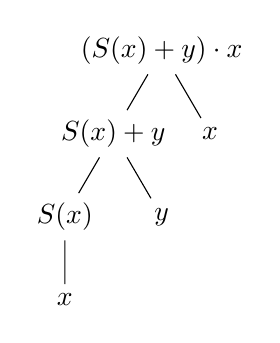
\begin{tikzpicture}[sibling distance=3.5em, level distance=3em]
  \node {$(S(x) + y)\cdot x$}
    child { node {$S(x)+y$} 
      child {node {$S(x)$}
      		child {node {$x$}}
      	}
      child {node {$y$}} }
    child { node {$x$} };
\end{tikzpicture}
\caption{A formation tree of the term $(S(x) + y)\cdot x$.}
\end{marginfigure}

The simplest type of formulas are the atomic formulas. These are only relations applied to terms. More formally, an \emph{atomic formula of a language $L$} is an expression $R(t_1, \dots, t_n)$, where $R$ is a relation symbol in $L$ and $t_1, \dots, t_n$ are terms of $L$. The set of all atomic formulas of a language $L$ is denoted as $\AFm_L$. Similarly to terms, atomic formulas can also be represented using formation trees from the formation trees of its terms and for binary relations, we use the infix notation, e.g. $\leq(x, y)$ can be written as $(x \leq y)$. For example $(x + y) = 0$, or $R(f(x), g(y,z), x)$ are atomic formulas ($f$ is a unary function, $g$ and $+$ are binary functions, and $R$ is a ternary relation).

We can finally define formulas in first-order language. The definition is similar to the one in propositional language, but this time the propositional variables are represented by atomic formulas and we additionally have the quantifiers. Formally, a \emph{formula of a language $L$} is defined inductively by
\begin{enumerate}
  \item Every atomic formula is a formula
  \item If $\varphi$ and $\psi$ are formulas, $(\varphi \to \psi), (\varphi \land \psi), (\varphi \lor \psi), (\varphi \lequiv \psi), (\neg \varphi)$ are also formulas.
  \item If $\varphi$ is a formula and $x \in \SVar$ is a variable, then $((\forall x)\varphi)$ and $((\exists x)\varphi)$ are formulas.
  \item Every formula is obtained by a finite application of the steps above.
\end{enumerate}

The set of all formulas of a language $L$ is denoted by $\Fm_L$. A formula that is a part of another formula $\varphi$ is a subformula of $\varphi$. Of course, formulas can also be expressed as their formation tree. An example is on the right.

\begin{marginfigure}[-6\baselineskip]
\centering
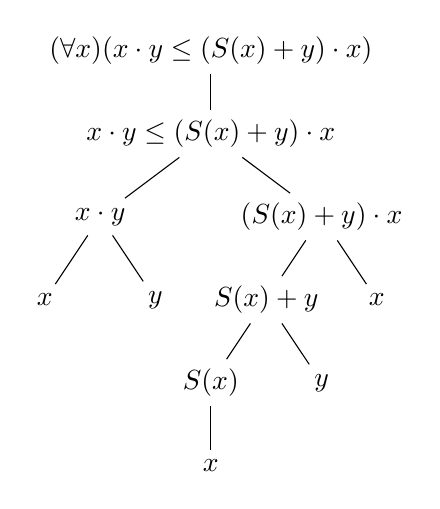
\begin{tikzpicture}[level 2/.style={sibling distance=8em}, 
                    level 3/.style={sibling distance=4em}, 
                    level distance=3em]
  \node {$(\forall x) (x \cdot y \leq (S(x) + y)\cdot x)$}
  	child {node {$x \cdot y \leq (S(x) + y)\cdot x$}
  		child {node {$x \cdot y$}
  			child {node {$x$}}
  			child {node {$y$}}
  		}
  		child {node {$(S(x) + y)\cdot x$}
  			child { node {$S(x)+y$} 
      		child {node {$S(x)$}
      			child {node {$x$}}
      		}
      	child {node {$y$}} 
      	}
      	child {node {$x$}}
      }
    };
\end{tikzpicture}
\caption{A formation tree of the formula $(\forall x) (x \cdot y \leq (S(x) + y)\cdot x)$. Moreover, $x\cdot y$ and $(S(x) + y)\cdot x$ are roots of formation trees of the terms included in the formula.}
\end{marginfigure}

As before, we can define some conventions to simplify writing the formulas. After introducing priorities of binary function symbols ($+, \cdot, \dots$) we can omit parenthesis in the infix notation of terms that are around a subterm formed by a symbol of higher priority. We also introduce the priority of logical connectives similar to the priorities in the propositional logic. The negation and quantifiers ($\neg, (\forall x), (\exists x)$) have the highest priorities, then we have conjunction and disjunction ($\land, \lor$) and, finally, the implication and equivalence ($\to, \lequiv$) have the lowest priority. Now, we can omit some of the parenthesis in the formulas.

In predicate logic, there is an important difference between so called free and bound (occurrences of) variables, as we deal with each type differently in the semantics. For a formula $\varphi$ and variable $x$, an \emph{occurrence of $x$ in $\varphi$} is a leaf labeled by $x$ in the formation tree of $\varphi$. The occurrence of $x$ in $\varphi$ is \emph{bound}, if it is in some subformula $\psi$ that starts with $(\forall x)$ or $(\exists x)$. Otherwise the occurrence is \emph{free}. A \emph{variable is free} in a formula, if it has at least one free occurrence in the formula and it is \emph{bound} if it has at least one bound occurrence. A variable can be both free and bound at the same time. For example, in the formula $x > 0 \lor (\forall x) (\exists y)(x > y)$ the variable $x$ is both free and bound, as its first occurrence is free and the second one is bound. We will use the notation $\varphi(x_1, \dots, x_n)$ to denote that $x_1, \dots, x_n$ are all the free variables in $\varphi$.

A formula is \emph{open}, if it contains no quantifiers. The set of all open formulas in a language $L$ will be denoted as $\OFm_L$. Obviously, $\AFm_L \subsetneq \OFm_L \subsetneq \Fm_L$. On the other hand, a formula is \emph{closed (a sentence)} if it has no free variables. A formula can be both closed and open at the same time, all terms of such formulas are ground terms.

In mathematics, we very often have general theorems and we later use them with a more specific substitutions. This can more formally be expressed by substituting terms for free variables in formulas, however, we need to be careful, as in some cases the substitution can change the meaning of the formula. For example, if we substituted the term $y$ for $x$ in $(\exists y) (x+y=1)$, we would change the original meaning of the formula ``there is a $y$ such that $y = 1-x$'' to a new meaning that says ``y is divisible by 2''. We want to avoid such situation while performing the substitution. Therefore, we define a term $t$ is \emph{substitutable} for a variable $x$ in a formula $\varphi$, if after the substitution of $t$ for all free occurrences of $x$, none of the variables of $t$ become bound in $\varphi$. The new formula is denoted as $\varphi(x/t)$ and we call it an \emph{instance of the formula $\varphi$} after a substitution of term $t$ for variable $x$. Alternatively, we can also define that $t$ is not substitutable for $x$ in $\varphi$ if $x$ has a free occurrence in a subformula of the form $(\exists y)\psi$ or $(\forall y) \psi$ for some variable $y$ in $t$.

We can also rename the quantified variables, but we again need to be careful. In this case, we would like to obtain an equivalent formula. Let $(Qx)\psi$ be a subformula of $\varphi$ where $Q$ is either $\forall$ or $\exists$ and $y$ is a variable. Then, if $y$ is substitutable for $x$ in $\psi$ and $y$ is not free in $\psi$, we can replace the subformula $(Qx)\psi$ with $(Qy)\psi(x/y)$ to obtain a \emph{variant} of $\varphi$ in subformula $(Qx)\psi$. A variant of $\varphi$ is obtained by variation of one or more subformulas of $\varphi$.

\informal{Creating variants in predicate logic serves some important purposes. One of them is, that we can easily transform any formula with a variable that is both free and bound into its variant, where each variable is ``pure'', i.e. only free or only bound. Moreover, we will very often create variants from formulas in order to fulfill assumptions such as ``variable $x$ is not free in $\varphi$''.}

\section{Semantics of first-order logic}

In propositional logic, models were defined as truth assignments. The truth assignment was enough to tell whether a proposition is true or false. In predicate logic, the situation is a bit more complex. First of all, the values of variables can be taken from a larger set than only $\{0,1\}$. Moreover, we need to define, what all the functions and relations mean. A natural representation of models in first-order logic is a mathematical structure. A structure is a set and a definition of functions and relations on this set. 

More formally, if we have a signature of a language $L = \langle \mathcal{R}, \mathcal{F} \rangle$ and a non-empty set $A$, a \emph{realization (interpretation) of a relation symbol} $R \in \mathcal{R}$ on the set $A$ is any relation $R^A \subseteq A^{\ar(R)}$. A realization of $=$ is the identity relation on $A$, i.e. $\mathrm{Id}_A = \{(x, x) | x \in A\}$. \emph{A realization (interpretation) of a function symbol} $f \in \mathcal{F}$ is any function $f^A: A^{\ar(f)} \to A$. Specifically, a realization of a constant symbol is some element of $A$. A \emph{structure for the language $L$} ($L$-structure) is a triple $\mathcal{A} = \langle A, \mathcal{R}^A, \mathcal{F}^A \rangle$, where $A$ is a non-empty set called the domain of the structure $\mathcal{A}$, $\mathcal{R}^A$ is a collection of realizations of the relation symbols on $A$, and $\mathcal{F}^A$ is a collection of realizations of function symbols on $A$. A structure of the language is also called a model of the language, and the class of all models of a language $L$ will be denoted as $M(L)$.

You probably already know different mathematical structures from other parts of mathematics, for example:
\begin{enumerate}
	\item $S = \struct{S, \leq}$ is an ordered set, where $\leq$ is reflexive, antisymmetric, and transitive binary relation,
	\item $G = \struct{V, E}$ is a graph,
	\item $\Int_p = \struct{\Int_p, +, -, 0}$ is the additive group of integers modulo $p$,
	\item $\Rat = \struct{\Rat, +, -, 0, 1}$ is the field of rational numbers,
	\item $\mathcal{P}(X) = \struct{\mathcal{P}(X), \setminus, \cap, \cup, \emptyset, X}$ is the set algebra over $X$, and
	\item $\Nat = \struct{\Nat, S, +, \cdot, 0, \leq}$ is the standard model of arithmetic.
\end{enumerate}
But also many other objects can be defined as structures, e.g. the finite automata or even databases.

We now aim to define the truth value of formulas in first-order logic. We already know, that a formula is constructed from atomic formulas, which are in turn constructed from terms. Therefore, in order to define the truth value of a formula, we need to start with the definition of the value of a term. Let $t$ be a term of $L = \struct{\cR, \cF}$ and $\cA = \struct{A, \cR^A, \cF^A}$ an $L$-structure. A \emph{variable assignment} over the domain $A$ is a function $e: \SVar \to A$. The \emph{value $t^A[e]$ of the term $t$} in the structure $\cA$ with respect to the assignment $e$ is defined inductively by 
\begin{enumerate}
	\item $x^A[e] = e(x)$, for $x \in \SVar$,
	\item $(f(t_1, \dots, t_n))^A[e] = f^A(t_1^A[e], \dots, t_n^A[e])$ for $f \in \cF$.
\end{enumerate}
For a constant symbol $c^A[e] = c^A$, i.e. the values of constants do not depend on the assignment $e$, and therefore also the value of ground terms does not depend on the assignment. Obviously, the value of a term $t$ depends only on the assignment of variables in $t$.

We now know, how to compute the values of individual terms, therefore, we can define the value of atomic formulas. Contrary to the values of terms, values of formulas are always from the set $\{0,1\}$. Let $\varphi$ be an atomic formula of $L = \struct{\cR, \cF}$ in the form $R(t_1, \dots, t_n)$, $\cA = \struct{A, \cR^A, \cF^A}$ is an $L$-structure and $e$ a variable assignment over $A$. The \emph{value $H^A_{at}(\varphi)[e]$ of the atomic formula $\varphi$} in the structure $\cA$ with respect to $e$ is $$H^A_{at}(\varphi)[e] = \twopartdefotherwise{1}{(t_1^A[e], \dots t_n^A[e]) \in R^A}{0}$$

Specifically, for the equality relation $=$, the only possible realization is $\mathrm{Id}_A$ and therefore $H^A_{at}(t_1=t_2)[e] = 1$, if $t_1^A[e]=t_2^A[e]$ and $0$ otherwise. We can again see that the value of a formula depends only on the assignment of variables in the formula and that the value of a ground formula does not depend on the assignment at all.

We can finally define the value of a general formula. The definition is quite long, but also very similar to the one in propositional logic. In fact, the only difference is in the last two cases. The atomic formulas in this case play the role of the propositional variables.

The value $H^A(\varphi)[e]$ of formula $\varphi$ in the structure $A$ with respect to $e$ is 
\begin{align*}
	H^A(\varphi)[e] & = H^A_{at}(\varphi)[e] \text{ if } \varphi \text{is atomic} \\
	H^A(\neg \varphi)[e] & = -_1(H^A(\varphi)[e])\\
	H^A(\varphi \land \psi)[e] & = \land_1(H^A(\varphi)[e], H^A(\psi)[e])\\
	H^A(\varphi \lor \psi)[e] & = \lor_1(H^A(\varphi)[e], H^A(\psi)[e])\\
	H^A(\varphi \to \psi)[e] & = \to_1(H^A(\varphi)[e], H^A(\psi)[e])\\
	H^A(\varphi \lequiv \psi)[e] & = \lequiv_1(H^A(\varphi)[e], H^A(\psi)[e])\\
	H^A((\forall x)\varphi)[e] & = \min_{a \in A}(H^A(\varphi)[e(x/a)])\\
	H^A((\exists x)\varphi)[e] & = \max_{a \in A}(H^A(\varphi)[e(x/a)])
\end{align*}
where $-_1, \land_1, \lor_1, \to_1, \lequiv_1$ are the functions given by the truth tables in the part on propositional logic and $e(x/a)$ is an assignment  assigning value $a$ to variable $x$ and otherwise identical to $e$. We can see that the value of a formula depends only on the assignment of free variables in the formula (we check all possible assignments for the bound variables in steps 7 and 8).

The structure $\cA$ satisfies the formula $\varphi$ if $H^A(\varphi) = 1$, we denote the fact as $\cA \vDash \varphi[e]$, otherwise we write $\cA \nvDash \varphi[e]$. We can easily check that all the following hold
\begin{align*}
\cA \vDash \neg \varphi[e] & \Leftrightarrow \cA \nvDash \varphi[e] \\
\cA \vDash (\varphi \land \psi)[e] & \Leftrightarrow \cA \vDash \varphi[e] \text{ and } \cA \vDash \psi[e]\\
\cA \vDash (\varphi \lor \psi)[e] & \Leftrightarrow \cA \vDash \varphi[e] \text{ or } \cA \vDash \psi[e]\\ 
\cA \vDash (\varphi \to \psi)[e] & \Leftrightarrow \cA \vDash \varphi[e] \text{ implies } \cA \vDash \psi[e]\\
\cA \vDash (\varphi \lequiv \psi)[e] & \Leftrightarrow \cA \vDash \varphi[e] \text{ if and only if } \cA \vDash \psi[e]\\
\cA \vDash (\forall x)(\varphi)[e] & \Leftrightarrow \cA \vDash \varphi[e(x/a)] \text{ for every } a \in A \\
\cA \vDash (\exists x)(\varphi)[e] & \Leftrightarrow \cA \vDash \varphi[e(x/a)] \text{ for some } a \in A
\end{align*}
Furthermore, if $t$ is substitutable for $x$ in $\varphi$, then for every structure $\cA$ and assignment $e$, $\cA \vDash \varphi(x/t)[e]$ if and only if $\cA \vDash \varphi[e(x/a)]$, where $a = t^A[e]$. If $\psi$ is a variant of $\varphi$ then $\cA \vDash \varphi[e]$ if and only if $\cA \vDash \psi[e]$.

As in propositional logic, we can generalize the notion above to validity in structure and in theory. Let $\varphi$ be a formula of a language $L$, and $\cA$ an $L$-structure. We say, that \emph{$\varphi$ is valid in $\cA$}, denoted as $\cA \vDash \varphi$, if $\cA \vDash \varphi[e]$ for every $e: \SVar \to A$. We also say that \emph{$\cA$ satisfies $\varphi$}. Otherwise, we write $\cA \nvDash \varphi$. The formula \emph{$\varphi$ is contradictory in $\cA$} if $\cA \vDash \neg \varphi$, i.e. if $\cA \nvDash \varphi[e]$ for every $e$.

We can easily check, that for any structure $\cA$ and formulas $\varphi, \psi$ the following holds:
\begin{align}
	\cA \vDash \varphi & \Rightarrow \cA \nvDash \neg \varphi \\
	\cA \vDash \varphi \land \psi & \Leftrightarrow \cA \vDash \varphi \text{ and } \cA \vDash \psi\\
	\cA \vDash \varphi \lor \psi & \Leftarrow \cA \vDash \varphi \text{ or } \cA \vDash \psi\\
	\cA \vDash \varphi & \Leftrightarrow \cA \vDash (\forall x)\varphi
\end{align}
Moreover, if $\varphi$ and $\psi$ are sentences, the implications in (1) and (3) are in fact equivalences. The last equivalence (4) also shows, that $\cA \vDash \varphi$ if and only if $\cA \vDash \psi$, where $\psi$ is the \emph{universal closure} of $\varphi$, i.e. the formula $(\forall x_1)(\forall x_1) \dots (\forall x_n)\varphi$, where $x_1, \dots, x_n$ are all the free variables of $\varphi$.

A \emph{theory} of a language $L$ is any set $T$ of formulas of $L$ (the \emph{axioms} of the theory). A \emph{model of a theory $T$} is an $L$-structure $\cA$ such that $\cA \vDash \varphi$ for every $\varphi \in T$. We also write $\cA \vDash T$ and say that $\cA$ satisfies $T$. The \emph{class of all models} of theory $T$ is $M(T) = \{\cA \in M(L) | \cA \vDash T\}$. A formula is \emph{valid in $T$} (true in $T$) ($T\vDash \varphi$) if $\cA \vDash \varphi$ for every model $\cA$ of $T$. Otherwise we write $T \nvDash \varphi$. A formula \emph{$\varphi$ is contradictory in $T$} if $T \vDash \neg \varphi$ and \emph{$\varphi$ is independent in $T$} if it is neither valid nor contradictory in $T$. For empty theory $T$, we can omit $T$ in the notation and $M(T)=M(L)$. In this case, ($\vDash T$) means that the formula $\varphi$ is \emph{logically valid} (\emph{a tautology}). A \emph{consequence of $T$} is the set $\theta^L(T)$ of all sentences of $L$ valid in $T$, i.e. $$\theta^L(T) = \{\varphi \in \Fm_L\ | T\vDash \varphi \text{ and } \varphi \text{ is a sentence}\}\,.$$

\informal{The definitions above should closely resemble those we saw in propositional logic, the main difference is in the definition of the model. In propositional logic, we could use truth assignments, while in predicate logic, the model is a structure. The structure, and its definitions of functions and relations in fact give the truth values to the atomic formulas. The atomic formulas then play the role of the propositional variables. Of course, in predicate logic, we also need to take care of the quantifiers, which brings another complexity to the definitions.}

For example, the theory of orderings $T$ is a theory in language $L=\struct{\leq}$ with axioms
\begin{align*}
	x \leq x & & \text{reflexivity,} \\
	x \leq y \land y \leq x \to x = y & & \text{antisymmetry,} \\
	x \leq y \land y \leq z \to x \leq z & & \text{transitivity.} \\
\end{align*}

The models of $T$ (ordered sets) are structures $\struct{S, \leq_S}$. For example $\mathcal{A} = \struct{\Nat, \leq}$ or $\mathcal{B} = \struct{\mathcal{P}(X), \subseteq}$ for a set $X = \{0,1,2\}$. The formula $\varphi \equiv x \leq y \lor y \leq x$ is valid in $\cA$, but not in $\mathcal{B}$, as $\mathcal{B} \nvDash \varphi[e]$ for $e(x) = \{0\}$ and $e(y)=\{1\}$, therefore it is independent in $T$. The sentence $\psi \equiv (\exists x)(\forall y)(y \leq x)$ is valid in $\mathcal{B}$ and contradictory in $\cA$, and therefore also independent in $T$. Finally, the formula $\chi \equiv (x \leq y \land y \leq z \land z \leq x) \to (x = y \land y = z)$ is valid in $T$, denoted as $T \vDash \chi$.

We say that a theory $T$ in a language $L$ is \emph{semantically inconsistent} if $T \vDash \bot$, otherwise \emph{$T$ is consistent}. The theory \emph{$T$ is complete}, if it is consistent, and every sentence of $L$ is either valid or contradictory in $T$. The $L$-theory \emph{$T$ is an extension} of another theory $T'$ in language $L'$ if $L' \subseteq L$ and $\theta^{L'}(T') \subseteq \theta^L(T)$. The \emph{extension is simple}, if $L' = L$ and it is \emph{conservative} if $\theta^{L'}(T') = \theta^L(T) \cap \Fm_{L'}$. The \emph{two theories are equivalent}, if one is the extension of the other and vice versa.

We also define a form of equivalence for two structures -- we say that two $L$-structures $\cA, \cB$ are \emph{elementarily equivalent}, denoted as $\mathcal{A} \equiv \mathcal{B}$ if they satisfy the same sentences of $L$. It means that we cannot write a sentence in the language that would make any distinction between the two structures. Later, we will also define the isomorphism of structures and we will see that it is a stronger property, i.e. that any two isomorphic structures are elementarily equivalent, but not vice versa.

The definitions above lead to a simple observation -- a theory $T$ of language $L$ is consistent if it has a model. It is complete if and only if it has a single model, up to elementary equivalence. The theory $T$ is an extension of another theory $T'$ in the same language $L$ if and only if $M(T) \subseteq M(T')$ and the theories are equivalent if $M(T) = M(T')$.

We can transform the problem of validity in a theory into the problem of satisfiability of another theory, similarly to the proof by contradiction. For every theory $T$ and sentence $\varphi$ (in the same language), it holds $T \cup \{\neg \varphi\}$ is unsatisfiable if and only if $T \vDash \varphi$. Why? Because by the definitions, $T \cup \{\neg \varphi\}$ is unsatisfiable (i.e. has no model) if $\neg \varphi$ is not valid in any model of $T$, which means (and here we need the assumption that $\varphi$ is a sentence) that $\varphi$ is valid in every model of $T$ and that in turn means $T \vDash \varphi$. 

You also probably know the notion of substructure from other parts of mathematics. Let $\cA = \struct{A, \cR^A, \cF^A}$ and $\mathcal{B} = \struct{B, \cR^B, \cF^B}$ be structures for $L = \struct{\cR, \cF}$. We say that \emph{$\mathcal{B}$ is an (induced) substructure of $\cA$} ($\mathcal{B} \subseteq \cA$) if $B \subseteq A$, $R^B = R^A \cap B^{\ar(R)}$ for every $R \in \cR$, and $f^B = f^A \cap (B^{\ar(f)}\times B)$ for every $f \in \cF$. A set $C$ is a domain of some substructure of $\cA$ if and only if it is closed under all functions of $\cA$\sidenote{A set $C \subseteq A$ is closed under a function $f: A^{\ar(f)} \to A$, if $f(x_1, \dots, x_{ar(f)}) \in C$ for all $x_1, \dots, x_{\ar(f)} \in C$.}. The representative substructure is then called a \emph{restriction of $\cA$ to $C$} and denotes as $\cA \restrict C$.

If we have a structure $\cA$, its substructure $\mathcal{B}$ in a language $L$ and a value assignment $e: \SVar \to B$, then, obviously, for an open formula $\varphi$, $\cA \vDash \varphi[e]$ if and only if $\mathcal{B} \vDash \varphi[e]$. The essential fact here is that $e$ assigns only values from $B$ and therefore the values of the terms are the same in both $\cA$ and $\mathcal{B}$. The same then holds for the atomic formulas and by induction on the complexity of the formula also for general formulas. This simple observation however has an interesting corollary. For every open formula $\varphi$ and a structure $\cA$, the formula is valid in the structure $\cA$ if and only if it is valid in every substructure $\mathcal{B}$ of $\cA$. If a theory $T$ contains only open axioms (so called \emph{open theory}), this implies that every substructure of a model of $T$ is also a model of $T$.

The last observation is important in case we want to check, whether a theory $T$ is openly axiomatizable, i.e. if there is an equivalent theory $T'$ that contains only open axioms. In such a case, we just need to check, if every substructure of a model of the theory $T$ is also a model of $T$. If it is, then $T$ is openly axiomatizable, otherwise it is not.

Let $\cA = \struct{A, \cR^A, \cF^A}$ be a structure and $X \subseteq A$. Let $B$ be the smallest subset of $A$ containing $X$ and closed under all functions of $\cA$ (including constants). Then the structure $\cA \restrict B$ is denoted as $\cA\langle X \rangle$ and is called \emph{a substructure of $\cA$ generated by the set $X$}. 

Let $\cA$ be a structure for the language $L$ and $L'\subseteq L$. By omitting realizations of symbols that are not in $L'$ we obtain a structure $\cA'$ in $L'$ called the reduct of $\cA$ to the language $L'$. The structure $\cA$ is then called the expansion of $\cA'$ into $L$.

\chapter{Tableau method in first-order logic}

As in the propositional logic, we will use the tableau method to prove formulas in first order logic. While most of the ideas from propositional logic will be used again, the more complex structure of first-order formulas leads to additional rules in the tableau method (these are basically the atomic tableaux for the quantifiers). Also, the proofs of soundness and completeness will get more technical because we know need to also consider the structure of the terms, and because the models in first-order logic are mathematical structures rather than truth assignments. However, we will define so called canonical structure as a general structure for a language that prescribes the definitions of all function symbols, thus we will again need to define only the truth values of atomic formulas, thus reducing most of the ideas to propositional logic.

In fact, propositional logic can be seen as a fragment of the predicate logic, where we do not use the quantifiers and the propositional variables are represented by nullary predicate symbols.

In the tableau proofs in the predicate logic, we will work in a language that contains countable amount of new constants. Therefore it is important to show, that adding new constants to the language does not change the validity of formulas in the language. This should be intuitive -- adding constants without telling anything about them means we only add symbols that can be used as names of specific elements in the structure. This is more formally demonstrated by the following theorem.

\begin{theorem}
Let $\varphi$ be a formula in a language $L$ with free variables $x_1, \dots, x_n$ and let $T$ be a theory in $L$. Let $L'$ be an extension of $L$ with new constant symbols $c_1, \dots, c_n$ and let $T'$ denote the theory $T$ in $L'$. Then $$T \vDash \varphi \text{ if and only if } T'\vDash \varphi(x_1/c_1, \dots, x_n/c_n)\,.$$
\end{theorem}
\begin{proof}
($\Rightarrow$) If $\cA'$ is a model of $T'$, let $\cA$ be reduct of $\cA'$ to $L$. Since $\cA \vDash \varphi[e]$ for every assignment $e$, we have $\cA \vDash \varphi[e(x_1/c_1^{A'}, \dots, x_n/c_n^{A'})]$, i.e. $\cA' \vDash \varphi(x_1/c_1, \dots, x_n/c_n)$.

($\Leftarrow$) For the other implication, if $\cA$ is a model of $T$ and $e$ an assignment, let $\cA'$ be the expansion of $\cA$ into $L'$ by setting $c_i^{A'} = e(x_i)$ for every $i$. Since $\cA' \vDash \varphi(x_1/c_1, \dots, x_n/c_n)[e']$ for every assignment $e'$, we have $\cA' \vDash \varphi[e(x_1/c_1^{A'}, \dots, x_n/c_n^{A'})]$, i.e. $\cA \vDash \varphi[e]$.
\end{proof}

The basics of the tableau method in predicate logic are similar to the tableau method in propositional logic. A tableau is still a binary tree that represents the search for a counterexample. The nodes are still labeled with entries, i.e. formulas with a sign $T$ or $F$. However, this time, the formulas will be sentences. A branch is still contradictory if it contains $T \varphi$ and $F \varphi$ for a formula $\varphi$. A proof of a formula $\varphi$ is still a contradictory tableau with $F \varphi$ as its root entry. If a counterexample exists, there will be a non-contradictory branch in the finished tableau that provides us with the counterexample. We will again define a systematic tableau that is always finished and in case it is a proof of a formula, it is also finite. 

There are however some differences -- we need to add atomic tableaux for the logical quantifiers. In these the quantified variables will be substituted with ground terms following some rules. We extend the language by new constant symbols that act as the witnesses of the entries $T(\exists x) \varphi x$ and $F(\forall x) \varphi(x)$. In a finished non-contradictory branch for an entry $T (\forall x) \varphi(x)$, we will have the entries $T \varphi(x/t)$ for every ground term $t$ of the extended language. Similarly for $F (\forall x) \varphi(x)$ and $F \varphi(x/t)$.

We have some assumptions in the tableau method in predicate logic. First of all, the formula we want to prove needs to be a sentence. This is not a problem -- we can always prove the universal closure of a formula if it has free variables, as we already know, that these two are equivalent. Furthermore, we also assume the axioms of the theory are sentences -- but that is also not a problem, we can again take the universal closures of the axioms. We also assume that the language $L$ is countable. That also means that every theory in $L$ is countable. We define $L_C$ as the extension of $L$ by new constant symbols $c_0, c_1, \dots$. Then there are countably many ground terms of $L_C$. Let $t_i$ denote the $i$-th ground term in some fixed enumeration. Finally, we start with the assumption that $L$ is without equality, but we will deal with this one later.

\begin{figure*}[ht]
\centering
\begin{minipage}{\textwidth}
\begin{tabular}{|c|c|c|c|c|c|}
\hline
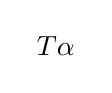
\begin{tikzpicture}[sibling distance=3em, level distance=3em]
  \node {$T \alpha$};
\end{tikzpicture} &
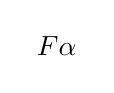
\begin{tikzpicture}[sibling distance=3em, level distance=3em]
  \node {$F \alpha$};
\end{tikzpicture} &
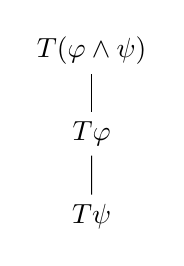
\begin{tikzpicture}[sibling distance=3em, level distance=3em]
  \node {$T (\varphi \land \psi)$}
    child { node {$T \varphi$} 
      child {node {$T \psi$}}};
\end{tikzpicture} &
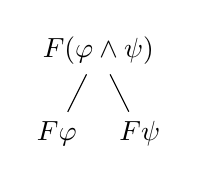
\begin{tikzpicture}[sibling distance=3em, level distance=3em]
  \node {$F (\varphi \land \psi)$}
    child { node {$F \varphi$} }
    child { node {$F \psi$}};
\end{tikzpicture} &
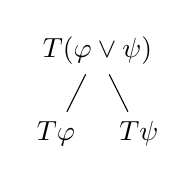
\begin{tikzpicture}[sibling distance=3em, level distance=3em]
  \node {$T (\varphi \lor \psi)$}
    child { node {$T \varphi$} }
    child { node {$T \psi$}};
\end{tikzpicture} &
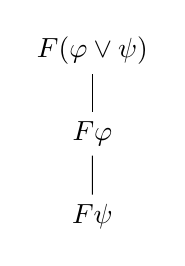
\begin{tikzpicture}[sibling distance=3em, level distance=3em]
  \node {$F (\varphi \lor \psi)$}
    child { node {$F \varphi$} 
      child {node {$F \psi$}}};
\end{tikzpicture} \\
\hline
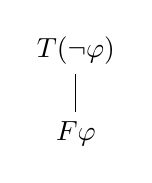
\begin{tikzpicture}[sibling distance=3em, level distance=3em]
  \node {$T (\neg \varphi)$}
    child { node {$F \varphi$} };
\end{tikzpicture} &
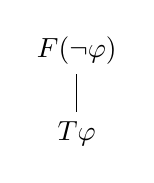
\begin{tikzpicture}[sibling distance=3em, level distance=3em]
  \node {$F (\neg \varphi)$}
    child { node {$T \varphi$} };
\end{tikzpicture} &
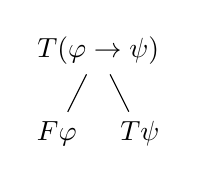
\begin{tikzpicture}[sibling distance=3em, level distance=3em]
  \node {$T (\varphi \to \psi)$}
    child { node {$F \varphi$} }
    child { node {$T \psi$}};
\end{tikzpicture} &
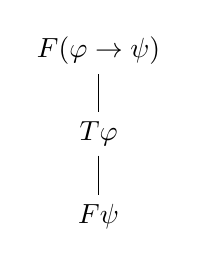
\begin{tikzpicture}[sibling distance=4em, level distance=3em]
  \node {$F (\varphi \to \psi)$}
    child { node {$T \varphi$} 
      child {node {$F \psi$}}};
\end{tikzpicture} &
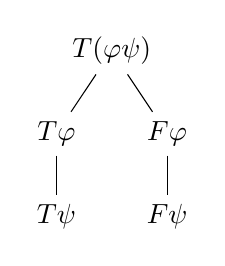
\begin{tikzpicture}[sibling distance=4em, level distance=3em]
  \node {$T (\varphi \lequiv \psi)$}
    child { node {$T \varphi$} 
    	child {node {$T \psi$}}}
    child { node {$F \varphi$} 
    	child {node {$F \psi$}}};
\end{tikzpicture} &
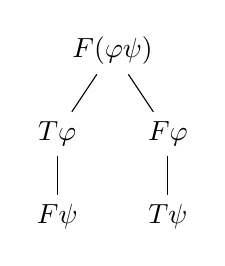
\begin{tikzpicture}[sibling distance=4em, level distance=3em]
  \node {$F (\varphi \lequiv \psi)$}
    child { node {$T \varphi$} 
    	child {node {$F \psi$}}}
    child { node {$F \varphi$} 
    	child {node {$T \psi$}}};
\end{tikzpicture} \\
\hline
\end{tabular}
\end{minipage}
\caption{The atomic tableaux for logical connectives. In the tableau, $\varphi, \psi$ are sentences and $\alpha$ are atomic sentences.}
\label{fig:pred_tableaux}
\end{figure*}

The tableaux will again be constructed from atomic tableaux. In the predicate logic, we still have the atomic tableaux for the logical connectives ($\lor, \land, \neg, \to, \lequiv$). These are essentially the same as in propositional logic, but instead of having tableaux for propositional variables, we have them for atomic sentences $\alpha$. These atomic tableaux are shown in Figure~\ref{fig:pred_tableaux}. In the tableaux, $\varphi$ and $\psi$ denote formulas in $L_C$, and $\alpha$ denotes an atomic sentence in the same language.

Additionally, we also have atomic tableaux for the quantifiers. These are shown in Figure~\ref{fig:pred_tableaux_quant}. Again, $\varphi$ represents a formula of the language $L_C$ with a free variable $x$, $t$ is any ground term of $L_C$ and $c$ is a new constant symbol from $L_C \setminus L$.

\begin{figure*}[ht]
\begin{minipage}{\textwidth}
\begin{tabular}{|c|c|c|c|}
\hline
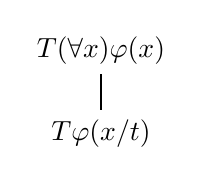
\begin{tikzpicture}[sibling distance=3em, level distance=3em]
  \node {$T (\forall x) \varphi(x)$}
  	child {node {$T \varphi(x/t)$}};
\end{tikzpicture} &
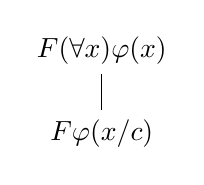
\begin{tikzpicture}[sibling distance=3em, level distance=3em]
  \node {$F (\forall x) \varphi(x)$}
  	child {node {$F \varphi(x/c)$}};
\end{tikzpicture} &
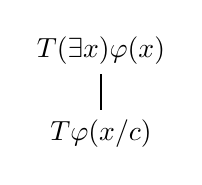
\begin{tikzpicture}[sibling distance=3em, level distance=3em]
  \node {$T (\exists x) \varphi(x)$}
  	child {node {$T \varphi(x/c)$}};
\end{tikzpicture} &
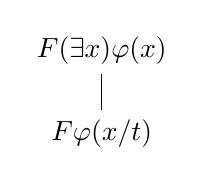
\begin{tikzpicture}[sibling distance=3em, level distance=3em]
  \node {$F (\exists x) \varphi(x)$}
  	child {node {$F \varphi(x/t)$}};
\end{tikzpicture} \\
for any term $t$ & for a new constant $c$ & for a new constant $c$ & for any term $t$ \\
\hline
\end{tabular}
\end{minipage}
\caption{The atomic tableaux for quantifiers}
\label{fig:pred_tableaux_quant}
\end{figure*}

The constant symbol $c$ represents a witness for the entry $T(\exists x)\varphi(x)$ or $F(\forall x)\varphi(x)$. These symbols must be new, i.e. not used anywhere else on the same branch in the tableau and also cannot be from the language $L$, as we do not want to assume anything about their value.

A \emph{tableau from a theory $T$} is again a sequence $\tau_0, \tau_1, \dots$ of finite tableaux from $T$, such that $\tau_{i+1}$ is formed from $\tau_i$ by steps 2 or 3 bellow, formally $\tau=\cup \tau_n$.

A \emph{finite tableau from a theory $T$} is a binary tree labeled with entries defined inductively as
\begin{enumerate}
 \item every atomic tableau from $T$ is a finite tableau from $T$, in cases $F(\forall x) \varphi(x)$ and $T(\exists x)\varphi(x)$ we may use any constant symbol $c \in L_C \setminus L$;
 \item if $P$ is an entry on a branch $V$ in a finite tableau from $T$ then by adjoining the atomic tableau from $P$ at the end of the branch $V$ we obtain a finite tableau from $T$, in cases $F(\forall x) \varphi(x)$ and $T(\exists x)\varphi(x)$ we may only use constant symbols $c \in L_C \setminus L$ that does not appear on $V$;
 \item if $V$ is a branch in a finite tableau from $T$ and $\varphi \in T$, then by adjoining $T \varphi$ at the end of $V$ we obtain a finite tableau from $T$; and
 \item every finite tableau is formed by finitely many steps above.
\end{enumerate}

Similarly to the tableau method in propositional logic, we do not need to repeat the entry that is expanded again on the branch. However, we have to repeat it in cases the entry is $T(\forall x) \varphi(x)$, or $F(\exists x)\varphi(x)$. This convention is demonstrated in the tableaux in Figure~\ref{fig:tableau_convention}.

\begin{figure}[ht]
\begin{minipage}{0.5\textwidth}
\centering
\begin{tikzpicture}[sibling distance=4em, level distance=3em]
  \node(n) {$F((\exists x)\neg P(x) \to \neg (\forall x)P(x))$}
    child { node {$T (\exists x)\neg P(x)$} 
    	child { node {$F \neg (\forall x)P(x)$} 
    		child {node {$F \neg (\forall x)P(x)$}
    			child {node {$T (\forall x)P(x)$}
    				child {node {$T (\exists x)\neg P(x)$}
	    				child {node {$T\neg P(c)$}
	    					child {node {$T\neg P(c)$}
	    						child {node {$F P(c)$}
	    							child {node {$T (\forall x)P(x))$}
	    								child {node {$T P(c)$}
	    									child {node {$\otimes$}}
	    								}
	    							}
	    						}
	    					}
	    				}
	    			}
    			}
    		}
    	}
    };
  \node[fit=(n)(n-1-1), draw] {};
  \node[fit=(n-1-1-1)(n-1-1-1-1), draw] {};
  \node[fit=(n-1-1-1-1-1)(n-1-1-1-1-1-1), draw] {};
  \node[fit=(n-1-1-1-1-1-1-1)(n-1-1-1-1-1-1-1-1), draw] {};
  \node[fit=(n-1-1-1-1-1-1-1-1-1)(n-1-1-1-1-1-1-1-1-1-1), draw] {};
\end{tikzpicture}
\end{minipage}
\begin{minipage}{0.5\textwidth}
\centering
\begin{tikzpicture}[sibling distance=4em, level distance=3em]
  \node(n) {$F((\exists x)\neg P(x) \to \neg (\forall x)P(x))$}
    child { node {$T (\exists x)\neg P(x)$} 
    	child { node {$F \neg (\forall x)P(x)$} 
  			child {node {$T (\forall x)P(x)$}
					child {node {$T\neg P(c)$}
						child {node {$F P(c)$}
							child {node {$T (\forall x)P(x))$}
								child {node {$T P(c)$}
									child {node {$\otimes$}}
								}
							}
						}
					}
    		}
    	}
    };
    \node[fit=(n-1-1-1-1-1-1)(n-1-1-1-1-1-1-1), draw] {};
\end{tikzpicture}
\end{minipage}
\caption{Example tableau. The rectangles on the left show the atomic tableaux used. The version on the right removes the repeated entries that can be removed, the entry in the rectangle in the right tableau must be repeated. $c$ is a new constant symbol where it first appears in the tableau, and in the last step, we chose $c$ as the term in the atomic tableau for $T(\forall x)P(x)$. The symbol $\otimes$ denotes a contradictory branch.}
\label{fig:tableau_convention}
\end{figure}

\informal{The cases where we need to repeat the entry are those where we can choose any term in the atomic tableau and if we chose incorrectly, we want to have another attempt to guess correctly. By repeating the entry on the branch, we have another non-reduced entry of the same type that we will reduce later.}

A \emph{branch $V$ is contradictory} if it contains entries $T \varphi$ and $F \varphi$ for some sentence $\varphi$, otherwise it is noncontradictory. A tableau $\tau$ is contradictory if all its branches are contradictory. A \emph{tableau proof of a sentence $\varphi$ from $T$} is a contradictory tableau from $T$ with $F \varphi$ in the root. $T \vdash \varphi$ denotes that $\varphi$ is tableau provable from $T$. A \emph{refutation of a sentence $\varphi$ by a tableau from $T$} is a contradictory tableau from $T$ with $T \varphi$ in the root. A sentence is tableau refutable if there is a tableau refutation of the sentence.

Compared to the propositional version of the tableau method, the definition of a finished tableau is a bit more complicated -- we need to account for the cases where we need to guess the correct terms and such atomic tableaux must be in the tableau for all the ground terms of $L_C$. This is reflected in the definition of the reduced entry. An occurrence on an entry $P$ in a node $v$ of a tableau $\tau$ is $i$-th if $v$ has exactly $i-1$ predecessors labeled by $P$. The \emph{occurrence of $P$ is reduced}, if $P$ is neither of in form $T(\forall x)\varphi(x)$ nor $F(\exists x)\varphi(x)$ and $P$ occurs in $V$ as a root of an atomic tableau (it was already expanded on $V$); or if $P$ is in form $T(\forall x)\varphi(x)$ or $F(\exists x)\varphi(x)$, $P$ has an $(i+1)$-th occurrence on $V$ and $V$ contains an entry $T \varphi(x/t_i)$ or $F \varphi(x/t_i)$, where $t_i$ is the $i$-th ground term in $L_C$ (in some enumeration of ground terms). Now, let $V$ be a branch in a tableau $\tau$ from a theory $T$. We say that $V$ is finished if it is contradictory, or every occurrence of an entry on $V$ is reduced on $V$, and moreover $V$ contains $T \varphi$ for every $\varphi \in T$. A tableau $\tau$ is finished if every branch in $\tau$ is finished.

We can now define the systematic tableau in predicate logic. The systematic tableau is again always finished and, moreover, if it is a proof, it is finite, as we shall see later. Let $R$ be an entry and $T=\{\varphi_0, \varphi_1, \dots\}$ a theory. The systematic tableau for $R$ from $T$ is the result $\tau = \cup \tau_n$ of the following construction:
\begin{enumerate}
  \item $\tau_0$ is the atomic tableau for $R$. In case $R$ is of the form $T(\exists x)\varphi(x)$ or $F(\forall x) \varphi(x)$ we take $c_0$ as the new constant. In case $R$ is of form $T(\forall x) \varphi(x)$ or $F(\exists x) \varphi(x)$ we take $t_1$ as the term.
  \item Let $v$ be the leftmost node in the smallest level as possible in tableau $\tau_n$ containing an occurrence of an entry $P$ that is not reduced on some noncontradictory branch through $v$.
  \item If $P$ is neither $T(\forall x)\varphi(x)$ nor $F(\exists x)\varphi(x)$, let $\tau'_n$ be the tableau obtained from $\tau_n$ by adjoining the atomic tableau for $P$ to every noncontradictory branch through $v$. In case $P$ is in the form $T(\exists x)\varphi(x)$ or $F(\forall x) \varphi(x)$, we take $c_i$ as the new constant for lowest possible $i$.
  \item If $P$ is either $T(\forall x)\varphi(x)$ or $F(\exists x)\varphi(x)$ and it has the $i$-th occurrence in $v$, let $\tau'_n$ be the tableau obtained from $\tau_n$ by adjoining the atomic tableau for $P$ to every noncontradictory branch through $v$, where we take the term $t_i$ for $t$.
  \item Let $t_{n+1}$ be the tableau obtained from $\tau'_n$ by adjoining $T \varphi_n$ to every noncontradictory branch that does not contain $T \varphi_n$ yet.
\end{enumerate}  

An example of a systematic tableau is shown in Figure~\ref{fig:tableau_systematic}.

\begin{figure}[t]
\centering
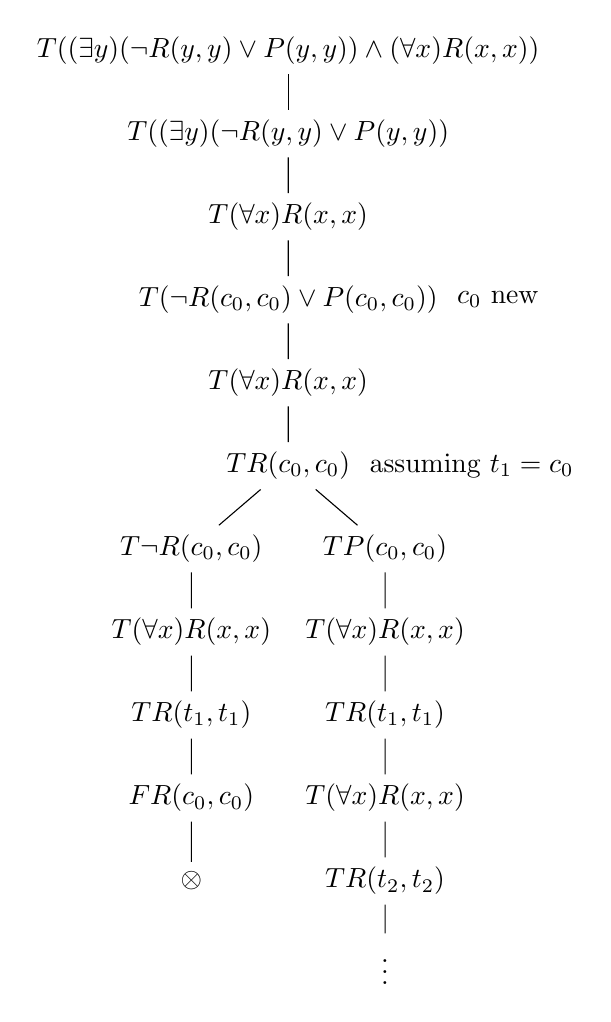
\begin{tikzpicture}[sibling distance=7em, level distance=3em]
  \node(n) {$T((\exists y)(\neg R(y,y) \lor P(y,y)) \land (\forall x)R(x,x))$}
    child { node {$T((\exists y)(\neg R(y,y) \lor P(y,y))$} 
    	child { node {$T(\forall x)R(x,x)$} 
    		child {node [label=right:{$c_0$ new}] {$T(\neg R(c_0,c_0) \lor P(c_0,c_0))$}
    			child {node {$T(\forall x)R(x,x)$}
    				child {node [label=right:{assuming $t_1 = c_0$}]{$TR(c_0,c_0)$}
	    				child {node {$T\neg R(c_0, c_0)$}
	    					child {node {$T(\forall x)R(x,x)$}
	    						child {node {$TR(t_1, t_1)$}
	    							child {node {$FR(c_0, c_0)$}
	    								child {node {$\otimes$}}
	    							}
	    						}
	    					}
	    				}
	    				child {node {$TP(c_0, c_0)$}
	    					child {node {$T(\forall x)R(x,x)$}
	    						child {node {$TR(t_1, t_1)$}
	    							child {node {$T(\forall x)R(x,x)$}
	    								child {node {$TR(t_2, t_2)$}
	    									child {node {$\vdots$}}
	    								}
	    							}
	    						}
	    					}
	    				}
	    			}
    			}
    		}
    	}
    };
\end{tikzpicture}
\caption{An example of a systematic tableau. The left branch is contradictory, while the right one is noncontradictory and finished but infinite.}
\label{fig:tableau_systematic}
\end{figure}


As in propositional logic, every systematic tableau is finished. We can show this using the same method as in propositional logic. Let $\tau = \cup \tau_n$ be a systematic tableau from $T = \{\varphi_0, \varphi_1, \dots\}$ with a root entry $R$ and let $P$ be an entry in a node $v$ of the tableau $\tau$. There are only finitely many entries in levels above $v$, therefore if the occurrence of $P$ in $v$ was unreduced, it would be eventually found in step 2, and reduced in steps 3 or 4 of the construction above. The step 4 above ensures that for every $\varphi_n \in T$, $T \varphi_n$ is in the tableau no later in $\tau_{n+1}$ on every noncontradictory branch. Therefore, all the branches in the tableau are finished.

We can also easily show that, if a systematic tableau $\tau$ is a proof (from a theory $T$), it is finite. Assume that $\tau$ is infinite, then by the König's lemma it contains an infinite branch. But this branch is noncontradictory, since we prolong only noncontradictory branches in the construction. But that is a contradiction with $\tau$ being a proof as proofs are contradictory tableaux.

Up until now, we have discussed tableau method only in languages without equality, however, the principles are the same in languages with equality, we just need to add the equality axioms into the theory. The \emph{equality axioms for language $L$} are 
\begin{enumerate}
	\item $x=x\,,$
	\item $x_1 = y_1 \land \dots \land x_n=y_n \to f(x_1, \dots, x_n) = f(y_1, \dots y_n)$ for every $n$-ary function symbol $f$ in $L\,,$ and
	\item $x_1 = y_1 \land \dots \land x_n=y_n \to (R(x_1, \dots, x_n) \to R(y_1, \dots y_n))$ for every $n$-ary relation symbol $R$ in $L$ (including ``='').
\end{enumerate}
The tableau proof from a theory $T$ in language $L$ with equality is a tableau proof from $T^*$ where $T^*$ denotes the extension of $T$ by adding the axioms of equality for $L$.

The problem is that the extended theory $T^*$ can have models, where equality is represented by a relation $=^A$ which is different from identity. This can be solved by considering the quotient structures by $=^A$ of these models. Let $\sim$ be an equivalence on $A$, $f: A \to A^n$, and $R\subseteq A^n$ for $n \in \Nat$. Then $\sim$ is a \emph{congruence for the function $f$} if for every $x_1, \dots, x_n, y_1, \dots, y_n \in A: x_1 \sim x_2 \land \dots \land x_n \sim y_n \Rightarrow f(x_1, \dots, x_n) \sim{=} f(y_1, \dots, y_n)$, and it is a \emph{congruence for the relation $R$} if for every $x_1, \dots, x_n, y_1, \dots, y_n \in A: x_1 \sim x_2 \land \dots \land x_n \sim y_n \Rightarrow R(x_1, \dots, x_n) \Leftrightarrow R(y_1, \dots, y_n)$. 

Let an equivalence $\sim$ in $A$ is a congruence for every function and relation in a structure $\cA = \struct{A, \cF^A, \cR^A}$ of language $L = \struct{\cF, \cR}$. The \emph{quotient structure of $\cA$ by $\sim$} is the structure $\quotient{\cA}{\sim} = \struct{\quotient{A}{\sim}, \cF^{\quotient{A}{\sim}}, \cR^{\quotient{A}{\sim}}}$ where
\begin{align*}
f^{\quotient{A}{\sim}}([x_1]_\sim, \dots [x_n]_\sim)&=[f^A(x_1, \dots, x_n)]_\sim \\
R^{\quotient{A}{\sim}}([x_1]_\sim, \dots, [x_n]_\sim) &\Leftrightarrow R^A(x_1, \dots, x_n)
\end{align*}
for each $f \in \cF, R \in \cR$, and $x_1, \dots, x_n \in A$. 

The axioms 1 and 3 of equality ensure that any relation $=^A$ that satisfies them is an equivalence, the axioms 2 and 3 ensure that the relation is also a congruence. If we have a model $\cA \vDash T^*$ then also ($\quotient{\cA}{=^A}) \vDash T^*$. Moreover, equality is interpreted as identity in $\quotient{\cA}{=^A}$.

We can now prove the soundness of the tableau method in predicate logic. The proof again closely resembles the one from the propositional logic. We will in fact also use a similar lemma. We say that a model $\cA$ agrees with an entry $P$ in a tableau if $P$ is $T \varphi$ and $\cA \vDash \varphi$ or if $P$ is $F \varphi$ and $\cA \vDash \neg \varphi$, i.e. $\cA \nvDash \varphi$. Moreover, $\cA$ agrees with a branch $V$ if $\cA$ agrees with every entry on $V$.

\begin{lemma}
Let $\cA$ be a model of a theory $T$ of a language $L$ that agrees with the root entry $R$ in a tableau $\tau = \cup \tau_n$ from $T$. Then $\cA$ can be expanded to a language $L_C$ so that it agrees with some branch $V$ in $\tau$.
\end{lemma}
\begin{proof}
We prove the lemma by induction on $n$. We will find a branch $V_n$ in $\tau_n$ and an expansion $\cA_n$ by constants $c^A$ for all $c \in L_C \setminus L$ on $V_n$ such that $\cA_n$ agrees with $V_n$ and $V_{n-1} \subseteq V_{n}$.

Assume we have a branch $V_n$ in $\tau_n$ and an expansion $\cA_n$ that agrees with $V_n$.
\begin{itemize}
	\item If $\tau_{n+1}$ is obtained from $\tau_n$ without extending the branch $V_n$, take $V_{n+1}=V_n$ and $\cA_{n+1}=\cA_n$.
	\item If $\tau_{n+1}$ is obtained from $\tau_n$ by appending $T \varphi$ for some $\varphi \in T$ to the end of $V_n$, let $V_{n+1}$ be the branch $V_n$ with $T \varphi$ at the end and $\cA_{n+1} = \cA_n$. Since $\cA \vDash \varphi$, $\cA_{n+1}$ agrees with $V_{n+1}$.
	\item Otherwise $\tau_{n+1}$ is obtained from $\tau_n$ by appending an atomic tableau for an entry $P$ on $V_n$ to $V_n$. By induction we know that $\cA$ agrees with $P$. If $P$ is formed by a logical connective, we take $\cA_{n+1}=\cA$ and verify that $V_n$ can always be extended to $V_{n+1}$ (this is the same as in propositional logic). If $P$ is in form $T(\forall x)\varphi(x)$, let $V_{n+1}$ be the unique extension of $V_n$ to a branch $\tau_{n+1}$ by the entry $T \varphi(x/t)$. Let $\cA_{n+1}$ be any expansion of $\cA_n$ by new constants from $t$. Since $\cA_n \vDash (\forall x) \varphi(x)$ also $\cA_{n+1} \vDash \varphi(x/t)$. Analogously for $P$ in form $F(\exists x) \varphi(x)$. Finally, if $P$ is in form $T(\exists x) \varphi(x)$, let $V_{n+1}$ be the unique extension of $V_n$ to a branch in $\tau_{n+1}$, i.e. by the entry $T \varphi(x/c)$. Since $\cA_n \vDash (\exists x) \varphi(x)$ there is some $a \in A$, such that $\cA \vDash \varphi(x)[e(x/a)]$ for every assignment $e$. Let $\cA_{n+1}$ be the expansion of $\cA_n$ by a new constant $c^A = a$. Then $\cA_{n+1} \vDash \varphi(x/c)$. Analogously for $P$ in form $F (\forall x)\varphi(x)$.
\end{itemize}
The base step for $n=0$ follows from the analysis of the atomic tableaux for the root entry $R$ applying the assumption that $\cA$ agrees with $R$.
\end{proof}

We can finally prove the soundness of the tableau method in first-order logic. The proof is in fact almost identical to the one in propositional logic. 

\begin{theorem}
For every theory $T$ and sentence $\varphi$, if $\varphi$ is tableau provable from $T$, then $\varphi$ is valid in $T$, i.e. $T \vdash \varphi \Rightarrow T \vDash \varphi$. 
\end{theorem}
\begin{proof}
Let $\varphi$ be tableau provable from $T$, i.e. there is a contradictory tableau from $T$ with root entry $F \varphi$. Assume for contradiction that $\varphi$ is not valid in $T$, i.e. there is a model $\cA$ of $T$ in which $\varphi$ is not true. However, in such a case $\cA$ agrees with the root entry $F \varphi$ of the proof and therefore by previous lemma it can be expanded to the language $L_C$ so that it agrees with a branch in $\tau$. But all the branches in $\tau$ are contradictory, thus it is not possible.
\end{proof}

Now, we would like to prove the completeness of the tableau method in first-order logic. We will again use the branch in a non-contradictory tableau and a model that agrees with the branch in order to provide a counter-example. This time, the model will be so called canonical model. In the canonical model, the universe is formed by all the ground terms of the language and the representations of all function symbols is fixed. This means we can imagine the ground atomic formulas, informally, as complex names of propositional variables and therefore the proof of completeness in principle reduces to its equivalent in the propositional logic.

Let $V$ be a noncontradictory branch of a finished tableau from a theory $T$ of a language $L = \struct{\cF, \cR}$. The \emph{canonical model} from $V$ is the $L_C$-structure $\cA = \struct{A, \cF^A, \cR^A}$ where $A$ is the set of all ground terms of the language $L_C$, $f^A(t_1, \dots, t_n) = f(t_1, \dots, t_n)$ for every $n$-ary function symbol $f \in \cF \cup (L_C \setminus L)$\sidenote{The expression $f(t_1, \dots, t_n)$ is a ground term of the language and therefore is in $A$.}, and $t_1, \dots, t_n \in A$, and $R^A(t_1, \dots, t_n) \Leftrightarrow TR(t_1, \dots, t_n)$ is an entry on $V$ for every $n$-ary relation symbol $R \in \cR$ and every $t_1, \dots, t_n \in A$.

If $L$ is with equality, $T^*$ is an extension of $T$ by the axioms of equality for $L$. The equality will be interpreted in the model by some relation $=^A$. We also have $t_1 =^A t_2 \Leftrightarrow T(t_1 = t_2)$ is an entry of $V$. Since $V$ contains all axioms of equality (it is finished), the relation $=^A$ is a congruence for all functions and relations in $\cA$. If we require that the equality is represented by identity, we take the quotient of the canonical model $\cA$ by the congruence $=^A$. The \emph{canonical model with equality} from $V$ is the quotient $\quotient{\cA}{=^A}$. 

\begin{lemma}
The canonical model $\cA$ from a noncontradictory finished branch $V$ agrees with $V$.
\end{lemma}
\begin{proof}
We will prove the lemma by induction on the structure of sentence $\varphi$ in an entry on $V$.
\begin{itemize}
	\item For atomic $\varphi$, if $T \varphi$ is on $V$ then $\cA \vDash \varphi$ by definition. If $F \varphi$ is on $V$, then $T \varphi$ is not on $V$ since $V$ is noncontradictory, so $\cA \vDash \neg \varphi$ by definition.
  \item If $T(\varphi \land \psi)$ is on $V$, then $T \varphi$ and $T \psi$ are on $V$ since $V$ is finished. By induction $\cA \vDash \varphi$ and $\cA \vDash \psi$, thus $\cA \vDash \varphi \land \psi$. For other logical connectives similarly (this step is the same as in the proof in propositional logic).
  \item If $T(\forall x) \varphi(x)$ is on $V$, then $T \varphi(x/t)$ is on $V$ for every term $t \in A$ since $V$ is finished. By induction $\cA \vDash \varphi(x/t)$ for every $t \in A$ and thus $\cA \vDash (\forall x) \varphi(x)$. Similarly for $F(\exists x) \varphi(x)$ on $V$.
  \item Finally, if $T(\exists x)\varphi(x)$ is on $V$, then $T \varphi(x/c)$ is on $V$ for some $c \in A$. By induction, $\cA \vDash \varphi(x/c)$ and thus $\cA \vDash (\exists x)\varphi(x)$. Similarly for $F(\forall x) \varphi(x)$ on $V$. 
\end{itemize}
\vspace{-\baselineskip}
\end{proof}

We can finally prove the completeness of the tableau method. As always, the proof is very similar to the one in propositional logic.

\begin{theorem}
For every theory $T$ and sentence $\varphi$, if $\varphi$ is valid in $T$, then $\varphi$ is tableau provable from $T$, i.e. $T \vDash \varphi \Rightarrow T \vdash \varphi$.
\end{theorem}
\begin{proof}
Let $\varphi$ is valid in $T$. We will show that an arbitrary finished tableau $\tau$ from a theory $T$ with the root entry $F \varphi$ is contradictory. Assume for a contradiction, that it is not, i.e. that there is a noncontradictory branch $V$ in $\tau$. By the previous lemma, there is a structure $\cA$ for $L_C$ that agrees with $V$, in particular with the root entry $F \varphi$, i.e. $\cA \vDash \neg \varphi$. Let $\cA'$ be the reduct of $\cA$ to the language $L$, then $\cA' \vDash \neg \varphi$. Since $V$ is finished, it contains $T \psi$ for every $\psi \in T$. Thus $\cA'$ is a model of $T$. But this contradicts the assumption that $\varphi$ is valid in $T$ ($\varphi$ is not valid in the model $\cA'$ of the theory $T$). Therefore the tableau $\tau$ is a proof of $\varphi$ from $T$.
\end{proof}

As with propositional logic, we can again re-define the semantical terms using syntactical notions. In fact, this and the next paragraph are copied from the propositional part with only minor changes. First of all, we define the \emph{set of theorems of $L$-theory $T$} $$\Thm^L(T) = \{\varphi | \varphi \in \Fm_L, T \vdash \varphi\}\,.$$ We say that a theory \emph{$T$ is inconsistent}, if $T \vdash \bot$, otherwise \emph{$T$ is consistent}. A theory \emph{$T$ is complete}, if it is consistent and every sentence is provable or refutable from $T$, i.e. if $T \vdash \neg \varphi$ or $T \vdash \varphi$. A theory $T$ in $L$ is \emph{an extension} of $T'$ in $L'$, if $L' \subseteq L$ and $\Thm^{L'}(T') \subseteq \Thm^{L}(T)$, the extension is \emph{simple}, if $L = L'$, and it is \emph{conservative} if $\Thm^{L'}(T') = \Thm^{L}(T) \cap \Fm_{L'}$. Two \emph{theories $T$ and $T'$ are equivalent}, if $T$ is an extension of $T'$ and vice versa.

There are strong relations between the syntactic terms introduced above and the semantic terms introduced in the previous chapter. Most of these are corollaries of the soundness and completeness of tableau method. For each theory $T$ and sentences $\varphi, \psi$ of a language $L$ 
\begin{enumerate}
	\item $T \vdash \varphi$ if and only if $T \vDash \varphi\,,$
	\item $\Thm^L(T) = \theta^L(T)\,,$
	\item $T$ is inconsistent if and only if $T$ is unsatisfiable, i.e. it has no model,
	\item $T$ is complete if and only if $T$ is semantically complete, i.e. it has a single model, up to elementary equivalence, and
	\item (deduction theorem) $T \cup \{\varphi\} \vdash \psi$ if and only if $T \vdash \varphi \to \psi\,.$
\end{enumerate}

A corollary of the proofs is the weak version of the Lövenheim-Skolem theorem.

\begin{theorem}
Every consistent theory $T$ of a countable language $L$ without equality has a countably infinite model.
\end{theorem}
\begin{proof}
Let $\tau$ be the systematic tableau from $T$ with $F\bot$ in the root. Since $\tau$ is consistent, $\bot$ is not provable from $T$ and therefore $\tau$ contains a noncontradictory branch $V$, and there exists a canonical model $\cA$ from $V$ (in language $L_C$). Since $\cA$ agrees with $V$ its reduct to the language $L$ is the desired countably infinite model of $T$.
\end{proof}

We needed the assumption that the theory is without equality because the canonical model with equality can be also finite (but it is always countable).

As in propositional logic, we can also prove the compactness theorem in first-order logic.

\begin{theorem}[compactness]
A theory $T$ has a model if and only if every finite subset of $T$ has a model.
\end{theorem}
\begin{proof}
The implication from left to right is obvious. For the other implication, if $T$ has no model, then it is inconsistent, i.e. $\bot$ is provable by a systematic tableau $\tau$ from $T$. Since $\tau$ is finite, $\bot$ is provable from some finite $T' \subseteq T$, i.e. $T'$ has no model.
\end{proof}

The compactness theorem has an interesting corollary which gives us the so call non-standard model of natural numbers. Let $\Nat = \struct{\Nat, S, +, \cdot, 0, \leq}$ be the standard model of natural numbers, and let $\Th(\Nat)$ be the theory consisting of all sentences valid in $\Nat$. For $n \in \Nat$, we denote $\underbar{n} = S(S(S(S(... S(0)))))$ ($n$ applications of the function $S$) the so called \emph{$n$-th numeral}. Now, let us consider a theory $T$ with a new constant symbol $c$, such that $T = \Th(\Nat) \cup \{\underbar{n} \lneq c | n \in \Nat\}$. Every finite subset of such theory has a model, therefore also the whole theory $T$ has a model. This is a \emph{non-standard model of natural numbers}. Every sentence that is valid in $\Th(\Nat)$ is also valid in this model, but it additionally contains an element that is greater than all natural numbers.

In mathematics, we very often define new functions or relations using formulas from the theory we work with. Now, we will show that such definitions do not in any way increase the strength of the theory, i.e. that by adding definitions of new symbols to a theory, we obtain a conservative extension of that theory. Before we get to that point, we will show a simple lemma that gives us a simple way to show that a theory is an (conservative) extension of another theory.

\begin{lemma}
Let $T$ be a theory of $L$ and $T'$ a theory of $L'$ where $L \subseteq L'$.
\begin{enumerate}
	\item $T'$ is an extension of $T$ if and only if the reduct $\cA$ of every model $\cA'$ of $T'$ to the language $L$ is a model of $T$,
	\item $T'$ is a conservative extension of $T$, if $T'$ is an extension of $T$ and every model $\cA$ of $T$ can be expanded to the language $L'$ on a model $\cA'$ of $T'$.
\end{enumerate}
\end{lemma}
\begin{proof}
\begin{enumerate}
  \item If $T'$ is an extension of $T$ and $\varphi \in T$ then $T' \vDash \varphi$. Thus $\cA' \vDash \varphi$ and also $\cA \vDash \varphi$, which implies that $\cA$ is a model of $T$. On the other hand, if $\cA$ is a model of $T$ and $T \vDash \varphi$ for a $\varphi$ of language $L$, then $\cA \vDash \varphi$ and also $\cA' \vDash \varphi$. Therefore $T' \vDash \varphi$ and $T'$ is an extension of $T$.
  \item If $T' \vDash \varphi$ where $\varphi$ is of the language $L$ and $\cA$ is a model of $T$, then in its expansion $\cA'$ that is a model of $T'$ we have also $\cA' \vDash \varphi$. Thus also $\cA \vDash \varphi$, and hence $T \vDash \varphi$. Therefore $T'$ is conservative.
\end{enumerate}
\vspace{-\baselineskip}
\end{proof}

We now start by showing that adding a definition of new relation does not change the strength of the theory. Let $T$ be a theory of a language $L$ and $\psi(x_1, \dots, x_n)$ a formula of $L$ with free variables $x_1, \dots, x_n$. Let $L'$ denote the extension of the language $L$ with a new $n$-ary relation symbol $R$. The \emph{extension of $T$ by definition of $R$} with a formula $\psi$ is the theory $T'$ of $L'$ obtained from $T$ by adding the axiom $R(x_1, \dots, x_n) \lequiv \psi(x_1, \dots, x_n)$. Obviously, in such a case every model of $T$ can be uniquely expanded into a model of $T'$ and therefore $T'$ is a conservative extension of $T$. Moreover, we can ``translate'' each formula $\varphi'$ of $L'$ into a formula $\varphi$ of $L$ such that $T' \vDash \varphi' \lequiv \varphi$. We just replace each sub-formula $R(t_1, \dots, t_n)$ with $\psi'(x_1/t_1, \dots, x_n/t_n)$, where $\psi'$ is a suitable variant of $\psi$ (such that every substitution can be performed).

Similarly, adding a definition of a function symbol does not increase the strength of the theory. Let $T$ be a theory of a language $L$, $\psi(x_1, \dots, x_n, y)$ an $L$-formula with free variables $x_1, \dots, x_n, y$ such that $T \vDash (\exists y)\psi(x_1, \dots, x_n, y)$ (existence) and $T \vDash \psi(x_1, \dots, x_n, y) \land \psi(x_1, \dots, x_n, z) \to y = z$ (uniqueness).
Let $L'$ be an extension of $L$ with a new $n$-ary function symbol $f$. The \emph{extension of $T$ by definition of $f$} by the formula $\psi$ is the theory $T'$ of $L'$ obtained from $T$ by adding the axiom $f(x_1, \dots, x_n) = y \lequiv \psi(x_1, \dots, x_n, y)$. Commonly, $\psi$ is $t(x_1, \dots, x_n) = y$ for a term $t$ and variables $x_1, \dots, x_n$. In such a case both existence and uniqueness always hold. Obviously, every model of $T$ can be uniquely extended to a model of $T'$ and therefore $T'$ is again a conservative extension of $T$. Moreover, we can again ``translate'' the formula $\varphi'$ in $L'$ into a formula $\varphi$ in $L$ such that these two formulas are $T'$-equivalent (i.e. $T' \vDash \varphi' \lequiv \varphi$). We show the translation only for formulas that contain the function $f$ only once, for other formulas, we can repeat the process inductively. Let $\varphi^*$ denote the formula obtained from $\varphi'$ by replacing the term $f(t_1, \dots, t_n)$ with a new variable $z$. Let $\varphi$ be the formula $(\exists z)(\varphi^* \land \psi'(x_1/t_1, \dots, x_n/t_n, y/z)$, where $\psi'$ is a suitable variant of $\psi$. Now, if $\cA$ is a model of $T'$, $e$ is an assignment, and $a = f^A(t_1, \dots, t_n)[e]$, by the two conditions, $\cA \vDash \psi'(x_1/t_1, \dots, x_n/t_n, y/z)[e]$ if and only if $e(z) = a$. Thus $\cA \vDash \varphi[e] \Leftrightarrow \cA \vDash \varphi^*[e(z/a)] \Leftrightarrow \cA \vDash \varphi'[e]$ for every assignment $e$, i.e. $\cA \vDash \varphi' \lequiv \varphi$ and so $T' \vDash \varphi' \lequiv \varphi$.

The two previous paragraphs show that if we have a theory $T'$ of the language $L'$ which was obtained from $T$ of $L$ by successive definitions of relation and function symbols (\emph{extension of $T$ by definitions}) then every model of $T$ can be uniquely expanded into a model of $T'$, $T'$ is a conservative extension of $T$, and for every formula $\varphi'$ of $L'$ there is a formula $\varphi$ of $L$ such that $T' \vDash \varphi' \lequiv \varphi$.

\chapter{Resolution in First-Order Logic}

We now aim to introduce the resolution method in predicate logic. To this end, we will need to show that the problem of satisfiability of theories can be reduced to open theories. We will show that every theory has an open conservative extension and therefore the satisfiability of the theory can be expressed as the satisfiability of the open extension. 

We say that two \emph{theories $T$ and $T'$ are equisatisfiable} it $T$ has a model if and only if $T'$ has a model. A formula is in the prenex (normal) form (PNF) if it is written as $(Q_1 x_1)\dots(Q_n x_n)\varphi'$, where $Q_i$ denotes $\forall$ or $\exists$ and $\varphi'$ is an open formula called the \emph{matrix}. $(Q_1 x_1)\dots(Q_n x_n)$ is the \emph{prenex}. If all the quantifiers are $\forall$ then $\varphi$ is a \emph{universal formula}.

We obtain the equisatisfiable open theory $T'$ by first transforming all axioms of $T$ into the prenex form. Then we remove the existential quantifiers (we will create so called Skolem variant of the formula) thus obtaining a universal formula. The matrices of the universal formulas will be the axioms of $T'$.

\section{Prenex Normal Form}

We start by the transformation of formulas into the prenex normal form. The transformation is based on replacing some occurrences of a sub-formula $\psi$ in a formula $\varphi$ by an equivalent sub-formula $\psi'$. It is easy to show (by induction on the structure of formula $\varphi$) that the obtained formula is equivalent to $\varphi$.

Let $Q$ denote $\forall$ or $\exists$ and $\bar{Q}$ denote the complementary quantifier. For every formulas $\varphi$ and $\psi$ such that $x$ is not free in the formula $\psi$, the following equivalences (\emph{conversion rules}) hold:
\begin{align*}
\neg(Qx)\varphi & \lequiv (\bar{Q}x)\neg \varphi \\
((Qx)\varphi \land \psi) & \lequiv (Qx)(\varphi \land \psi) \\
((Qx)\varphi \lor \psi) & \lequiv (Qx)(\varphi \lor \psi) \\
((Qx)\varphi \to \psi) & \lequiv (\bar{Q}x)(\varphi \to \psi) \\
(\psi \to (Qx) \varphi) & \lequiv (Qx)(\psi \to \varphi)
\end{align*}

All the equivalences can be proved by the tableau method. The assumption that $x$ is not free in $\psi$ is necessary in each rule above. 

By induction on the structure of formula $\varphi$, we can show that for every formula $\varphi$ there is an equivalent formula $\varphi'$ in the prenex normal form, i.e. $\vDash \varphi \lequiv \varphi'$. We just apply the conversion rules above (and replace subformulas with suitable variants if needed). 

\section{Skolem Variant}

If the prenex of the formula contains only universal quantifiers ($\forall$), we can remove them, thus obtaining an equivalent (and therefore also equisatisfiable) open formula. However, in many cases, some of the quantifiers will be existential. In such cases we can use the so called Skolem variant as the equisatisfiable formula.

Let $\varphi$ be a sentence of a language $L$ in the prenex normal form, let $y_1, \dots, y_n$ be the existentially quantified variables in $\varphi$ (in this order), and for every $i \leq n$ let $x_1, \dots, x_{n_i}$ be the universally quantified variables in $\varphi$ before $y_i$. Let $L'$ be an extension of $L$ with new $n_i$-ary function symbols $f_i$ for all $i \leq n$. Let $\varphi_S$ denote the formula obtained from $\varphi$ by removing all the $(\exists y_i)$ and replacing each occurrence of $y_i$ by $f_i(x_1, \dots, x_{n_i})$. Then $\varphi_S$ is the \emph{Skolem variant} of $\varphi$.

For example, for the formula $$(\exists y_1)(\forall x_1)(\forall x_2)(\exists y_2)(\forall x_3)R(x_1, y_1, x_2, y_2, x_3)$$ the Skolem variant is $$(\forall x_1)(\forall x_2)(\forall x_3)R(x_1, f_1, x_2, f_2(x_1, x_2), x_3)\,.$$ 

\informal{The new function symbols provide the witnesses for the existentially quantified variables. We need a function, as these can be different based on the previously universally quantified variables. That is also the reason, why the function have all the previously quantified variables as their parameters. The existentially quantified variables do not need to be included in the parameters, as the function can ``compute'' them from the universally quantified ones.}

We will now prove, that the Skolem variant $\varphi_S$ of $\varphi$ is equisatisfiable with $\varphi$. 

\begin{lemma}
Let $\varphi$ be a sentence $(\forall x_1)\dots(\forall x_n)(\exists y)\psi$ of $L$ and $\varphi'$ be a sentence $(\forall x_1)\dots(\forall x_n)\psi(y/f(x_1, \dots, x_n))$ where $f$ is a new function symbol. Then
\begin{enumerate}
	\item the reduct $\cA$ of every model $\cA'$ of $\varphi'$ to the language $L$ is a model of $\varphi$, and
	\item every model of $\varphi$ can be expanded into a model $\cA'$ of $\varphi'$.
\end{enumerate}
\end{lemma}
\begin{proof}
Let $\cA' \vDash \varphi'$ and $\cA$ be the reduct of $\cA'$ to $L$. Since $\cA \vDash \psi[e(y/a)]$ for every assignment $e$ where $a = (f(x_1, \dots, x_n)^{\cA'})[e]$, we have also $\cA \vDash \varphi$.

On the other hand, let $\cA \vDash \varphi$. There is a function $f^A: A^n \to A$ such that for every assignment holds $\cA \vDash \psi[e(y/a)]$ where $a = f^A(e(x_1), \dots, e(x_n))$, and thus the expansion $\cA'$ of $\cA$ by function $f^A$ is a model of $\varphi$.
\end{proof}

If $\varphi'$ is a Skolem variant of $\varphi$ then both statements above also hold and therefore $\varphi$ and $\varphi'$ are equisatisfiable.

It is important to realize that a formula and its Skolem variant are not equivalent. For example, $\varphi_S \equiv (\forall x)P(x,f(x))$ is a Skolem variant of $\varphi \equiv (\forall x)(\exists y)P(x,y)$. Let $\cA =\struct{\{0,1\}, P^A, f^A}$, where $P^A = \{(0,0), (1,1)\}$ and $f^A(0)=1, f^A(1)=0$. Then $\cA \vDash \varphi$, but $\cA \nvDash \varphi_S$. On the other hand, if $\varphi_S$ is valid in a structure, $\varphi$ also is, as $f$ gives the $y$ for which the formula holds, therefore, for a formula $\varphi$ and its Skolem variant $\varphi_S$, we always have $\vDash \varphi_S \to \varphi$. 

The difference between equivalence and equisatisfiability in this case is caused by the fact that the new functions in the Skolem variant are not in any way limited to cases where they provide the witnesses for the existence and can therefore be defined arbitrarily, as we saw above. If we defined the function in the ``intended'' way (in this case as the identity on $A$), the Skolem variant would hold in such a structure. Therefore, it is also satisfiable.

The transformation to prenex normal form and the following creation of Skolem variant gives us the possibility to reduce the question of satisfiability to open theories, i.e. for every theory, there is an equisatisfiable open theory. This is a corollary of the so called Skolem theorem.

\begin{theorem}[Skolem]
Every theory $T$ has an open conservative extension $T^*$.
\end{theorem}
\begin{proof}
We assume $T$ is in closed form (otherwise we can take the universal closures of all the axioms of $T$), and let $L$ be its language. We first replace each axiom of $T$ by an equivalent formula in prenex normal form, thus obtaining theory $T^\circ$. Next, we replace each axiom in $T^\circ$ by its Skolem variant, which gives us a theory $T'$ in a language $L' \supseteq L$. Since every reduct of every model of $T'$ to $L$ is a model of $T$, $T'$ is an extension of $T$. Furthermore, every model of $T$ can be expanded to a model of $T'$ and therefore $T'$ is a conservative extension of $T$. Every axiom of $T'$ is a universal sentence, therefore we can take the matrices of these sentences to obtain an open theory $T^\circ$ equivalent to $T'$. $T^\circ$ is the open conservative extension of $T$.
\end{proof}

\section{Herbrand Model}

We can even reduce the problem of satisfiability to propositional logic and show that if an open theory is unsatisfiable, we can demonstrate it via ground terms. For example, in the language $L = \struct{P, R, f, c}$ the theory $T=\{P(x,y) \lor R(x,y), \neg P(c,y), \neg R(x, f(x))\}$ is unsatisfiable because the following conjunction of finitely many ground instances of axioms of $T$ is unsatisfiable: $$P(c, f(c)) \lor R(c, f(c)) \land \neg P(c, f(c)) \land \neg R(c, f(c))\,.$$ This can also be seen as a unsatisfiable propositional formula $(p \lor r) \land \neg p \land \neg r$.

A \emph{ground instance} of formula $\varphi$ with free variables $x_1, \dots, x_n$ is $\varphi(x_1/t_1, \dots, x_n/t_n)$ where $t_1, \dots, t_n$ are ground terms.

The reduction of satisfiability to propositional logic is done using the notion of Herbrand models. Let $L = \struct{\cR, \cF}$ be a language with at least one constant symbol (we can add a new constant symbol, if needed). The \emph{Herbrand universe} for $L$ is the set of all ground terms of $L$. An $L$-structure $\cA$ is a \emph{Herbrand structure}, if its domain $A$ is the Herbrand universe for $L$ and for each $n$-ary function symbol $f \in \cF$, $t_1, \dots, t_n \in A$, $f^A(t_1, \dots, t_n) = f(t_1, \dots, t_n)$. A \emph{Herbrand model} of a theory $T$ is a Herbrand structure that is a model of $T$.

We can see, that the definition of the Herbrand universe and of the function symbols in the Herbrand structure is the same as in the canonical model, however, Herbrand structures do not specify the relations. This is important, as every canonical model is also a Herbrand model.

The reduction of unsatisfiability to propositional logic is formally given by the Herbrand's theorem.

\begin{theorem}[Herbrand]
Let $T$ be an open theory of a language $L$ without equality and with at least one constant symbol, then either $T$ has a Herbrand model, or there are finitely many ground instances of axioms of $T$ whose conjunction is unsatisfiable, and thus $T$ has no model.
\end{theorem}
\begin{proof}
Let $T'$ be the set of all ground instances of axioms of $T$. Consider a finished systematic tableau $\tau$ from $T'$ in the language $L$ (without adding new constant symbols) with the root entry $F \bot$. If the tableau $\tau$ contains a noncontradictory branch V, the canonical model from $V$ is a Herbrand model. Otherwise, $\tau$ is contradictory, i.e. $T' \vdash \bot$. Therefore $\tau$ is also finite and $\bot$ is provable from finitely many formulas of $T'$, i.e. their conjunction is unsatisfiable.
\end{proof}

The Herbrand model also works in languages $L$ with equality, we just need to take the extension $T^*$ of $T$ with the axioms of equality and if $T^*$ has a Herbrand model $\cA$ we take its quotient by $=^A$.

A corollary of the Herbrand's theorem is that an open theory $T$ of a language $L$ with at least one constant symbol is satisfiable if and only if the theory $T'$ of all ground instances of axioms of $T$ is satisfiable. Why? If $T$ has a model $\cA$, every instance of each axiom of $T$ is valid in $\cA$, and thus $\cA$ is also a model of $T'$. If $T$ is unsatisfiable then by Herbrand theorem there are finitely ground instances of axioms of $T$ that are not satisfiable and therefore $T'$ is also unsatisfiable.

Another corollary says that for every open $\varphi(x_1, \dots, x_n)$ of a language $L$ with at least one constant symbol, the formula $(\exists x_1)\dots(\exists x_n)\varphi$ is valid if and only if there exist $mn$ ground terms $t_{ij}$ of $L$ for some $m$ such that $\varphi(x_1/t_{11}, \dots, x_n/t_{1n}) \lor \dots \lor \varphi(x_1/t_{m1}, \dots, x_n/t_{mn})$ is a tautology. We know that $(\exists x_1)\dots(\exists x_n)\varphi$ is valid if and only if its negation $(\forall x_1)\dots(\forall x_n)(\neg\varphi)$ is unsatisfiable, which is equivalent to $\neg \varphi$ being unsatisfiable. The Herbrand theorem for $\{\neg \varphi\}$ gives us finitely many ($m$) ground instances of $\{\neg \varphi\}$ such that their conjunction $\psi$ is unsatisfiable. The negation of $\psi$ is the desired tautology.

We will now discuss the resolution method in predicate logic. It is again a refutation procedure, i.e. it aims to show that a formula or theory are not satisfiable. It assumes the formulas are open and in CNF. These are then represented in the clausal form as in propositional logic. Now, \emph{literals} are atomic formulas and their negations, \emph{a clause} is a finite set of literals ($\square$ denotes the empty clause) and a \emph{formula in clausal form} is a set of clauses. The resolution rule in first-order logic is based on the rule in propositional logic, but is more general -- it allows to resolve through literals that are different, if they are unifiable (i.e. if there is such a substitution that they become identical). Resolution in first-order logic is thus based on the resolution in propositional logic and unification.

\section{Resolution}

The Herbrand's theorem actually gives us an (ineffective) way, how to perform the resolution in first-order logic. If we have an input formula $S$ in clausal form and we assume the language has at least one constant symbol, we can create the set $S'$ of all ground instances of all clauses in $S$. If we know consider the atomic sentences as names of propositional variables, we may view $S'$ as a propositional formula in clausal form. We may now verify that it is unsatisfiable using the propositional version of the resolution method. While this method in principle works, it is very inefficient, as we need to work with large numbers of ground instances. Therefore, instead of grounding, we use suitable substitutions in order to perform the resolution on as general clauses as possible.

A \emph{substitution} is a finite set $\sigma = \{x_1/t_1, \dots, x_n/t_n\}$, where $x_i, i \leq n$ are distinct variables, $t_i$ are terms and the term $t_i$ is not $x_i$. If all $t_i$ are ground terms, $\sigma$ is a \emph{ground substitution}, if $t_i$ are distinct variables, $\sigma$ is a \emph{renaming of variables}. An \emph{instance of an expression $E$ by substitution $\sigma = \{x_1/t_1, \dots, x_n/t_n\}$} is the expression $E \sigma$ obtained from $E$ by simultaneously replacing all occurrences of $x_i$ by $t_i$. For a set $S$ of expressions, let $S \sigma = \{E \sigma| E \in S\}$. For two substitutions $\sigma = \{x_1/t_1, \dots, x_n/t_n\}$ and $\tau = \{y_1/s_1, \dots, y_m/s_m\}$ we define the \emph{composition of $\sigma$ and $\tau$} as $\sigma \tau = \{x_i/t_i \tau| x_i \in X, t_i \tau\text{ is not }x_i\} \cup \{y_j/s_j|y_j \in Y \setminus X\}\,$ where $X = \{x_1, \dots, x_n\}$ and $Y = \{y_1, \dots, y_m\}$. For every expression $E$ and substitutions $\sigma, \tau, \rho$ it holds (without proof) that $(E \sigma)\tau = E(\sigma \tau)$ and $(\sigma \tau)\rho = \sigma(\tau \rho)$.

A unification is a special substitution. Let $S = \{E_1, \dots, E_n\}$ be a finite set of expressions. A \emph{unification for $S$} is a substitution $\sigma$ such that $E_1 \sigma = E_2 \sigma = \dots = E_n \sigma$, i.e. $S \sigma$ is a singleton. We say that \emph{$S$ is unifiable}, if $S$ has a unification. A unification $\sigma$ of $S$ is a \emph{most general unification (mgu)} if for every unification $\tau$ of $S$ there is a substitution $\lambda$ such that $\tau = \sigma \lambda$. Obviously, if $\sigma$ and $\tau$ are two different most general unifications of $S$, they differ only in renaming of variables.

The general resolution rule in first-order logic is then defined in the following way: let $C_1, C_2$ be clauses with distinct variables such that $C_1 = C'_1 \sqcup \{A_1, \dots, A_n\}$ and $C_2 = C'_2 \sqcup \{\neg B_1, \dots, \neg B_m\}$, let $\sigma$ be a most general unifier of $S = \{A_1, \dots, A_n, B_1, \dots, B_m\}$. The \emph{resolvent} of $C_1$ and $C_2$ is $C = C'_1 \sigma \cup C'_2 \sigma$.

For example, in clauses $\{P(x), Q(x,z)\}$ and $\{\neg P(y), \neg Q(f(y), y)\}$ we can unify $S = \{Q(x,z), Q(f(y),y)\}$ applying the most general unification $\sigma = \{x/f(y), z/y\}$ and resolve to a clause $\{P(f(y)), \neg P(y)\}$.

The resolution proof and related notions are then defined in almost the same way as in propositional logic. Resolution proof (deduction) of a clause $C$ from a formula $S$ is a finite sequence $C_0, \dots, C_n = C$, such that for every $i \leq n$, we have $C_i = C'_i \sigma$ form some $C'_i \in S$ and a renaming of variables $\sigma$, or $C_i$ is a resolvent of some previous clauses. A clause $C$ is (resolution) provable from $S$ ($S \vdash_R C$), if it has a resolution proof from $S$. A refutation of a formula $S$ is a resolution proof of $\square$ from $S$. $S$ is resolution refutable if $S \vdash_R \square$.

It remains to show how to find the most general unifications we need in the resolution method. There is in fact a simple algorithm to find them: let $S$ be a finite set of expressions and $p$ be the leftmost position in which some expressions of $S$ differ. Then the difference in $S$ is the set $D(S)$ of subexpressions of all expressions of $S$ starting at the position $p$. For example $S = \{P(x,y), P((f(x), z), P(z, f(x)\}$ has $D(S) = \{x, f(x), z\}$.

The input of the algorithm is a nonempty finite set of expressions $S$, its output is the most general unification $\sigma$ of $S$ or information that $S$ is not unifiable. The algorithm performs the steps bellow:
\begin{enumerate}
	\item Let $S_0 \gets S, \sigma_0 \gets \emptyset, k \gets 0$.
	\item If $S_k$ is a singleton, output the substitution $\sigma = \sigma_0 \sigma_1 \dots \sigma_k$.
	\item If $D(S_k)$ contains a variable $x$ and a term $t$ with no occurrence of $x$, let $\sigma_{k+1} \gets \{x/t\}, S_{k+1} \gets S_k \sigma_{k+1}, k \gets k+1$ and go to step 2.
	\item Otherwise output ``S is not unifiable''.
\end{enumerate}

The occurrence check in step 3 can be expensive and slows the algorithm down significantly. Therefore some implementations (e.g. those in most Prolog interpreters) ignore that. However, it can lead to infinite loops.

We now show the correctness of the unification algorithm -- the unification algorithm outputs a correct answer in finite time for any input $S$, i.e. a most general unification $\sigma$ of $S$ or it detects that $S$ is not unifiable. The algorithm eliminates one variable in each iteration, therefore it finishes in finite time. If it ends negatively after $k$ iterations, $D(S_k)$ is not unifiable and therefore also $S$ is not. If it outputs $\sigma = \sigma_0 \sigma_1 \dots \sigma_k$, clearly $\sigma$ is a unification of $S$. We only need to show it is a most general one, i.e. for every unification $\tau$ of $S$ there is a substitution $\lambda$ such that $\tau = \sigma \lambda$. We will show that in this case, $\lambda = \tau$ and therefore $\tau = \sigma \tau$ (this property will also be important in the proof of lifting lemma later, let us call this property (*)). Let $\tau$ be a unification of $S$, we will show that $\tau = \sigma_0 \sigma_1 \dots \sigma_i \tau$ for every $i \leq k$. It obviously holds for $k = 0$. Let $\sigma_{i+1} = \{x/t\}$ and assume $\tau = \sigma_0 \sigma_1 \dots \sigma_i \tau$. It suffices to show that $v \sigma_{i+1} \tau = v \tau$ for every variable $\tau$. If $v \neq x$, $v \sigma_{i+1} = v$ and it holds. Otherwise $v = x$ and $v \sigma_{i+1} = x \sigma_{i+1} = t$. Since $\tau$ unifies $S_i=S \sigma_0 \sigma_1 \dots \sigma_i$ and both the variable $x$ and term $t$ are in $D(S_i)$ (otherwise $\sigma_{i+1}$ would be different), $\tau$ has to unify $x$ and $t$, i.e. $t \tau = x \tau$ as required.

\section{Soundness and Completeness}

In order to show the soundness of the resolution method, we first show the soundness of the general resolution rule.

\begin{lemma}
Let $C$ be a resolvent of clauses $C_1$ and $C_2$. For every $L$-structure $\cA$, if $\cA \vDash C_1$ and $\cA \vDash C_2$, then $\cA \vDash C$. 
\end{lemma}
\begin{proof}
Let $C_1 = C'_1 \sqcup \{A_1, \dots, A_n\}$ and $C_2 = C'_2 \sqcup \{\neg B_1, \dots, \neg B_m\}$, let $\sigma$ be a most general unifier of $S = \{A_1, \dots, A_n, B_1, \dots, B_m\}$, and let $C = C'_1 \sigma \cup C'_2 \sigma$. Since $C_1, C_2$ are open, also $\cA \vDash C_1 \sigma$ and $\cA \vDash C_2 \sigma$. We have $C_1 \sigma = C'_1 \sigma \cup \{S \sigma\}$ and $C_2 \sigma = C'_2 \cup \{\neg (S \sigma)\}$. We show $\cA \vDash C[e]$ for every assignment $e$. If $\cA \vDash S \sigma[e]$, then $\cA \vDash C'_2 \sigma[e]$, and thus $\cA \vDash C[e]$, otherwise $\cA \nvDash S \sigma [e]$, so $\cA \vDash C'_1 \sigma[e]$ and thus $\cA \vDash C[e]$.
\end{proof}

\begin{theorem}[soundness of resolution]
If $S$ is resolution refutable, then $S$ is unsatisfiable.
\end{theorem}
\begin{proof}
Let $S \vdash_R \square$. Suppose $\cA \vDash S$ for some structure $\cA$. By soundness of general resolution rule we also have $\cA \vDash \square$, which is not possible.
\end{proof}

The proof of completeness of resolution in predicate logic is based on its completeness in propositional logic. The connection between the propositional and predicate levels is given by the lifting lemma.

\begin{lemma}[lifting]
Let $C^*_1 = C_1 \tau_1$ and $C^*_2 = C_2 \tau_2$ be ground instances of clauses $C_1$ and $C_2$ with distinct variables and let $C^*$ be a resolvent of $C^*_1$ and $C^*_2$. Then there exists a resolvent $C$ of $C_1$ and $C_2$ such that $C^* = C \tau_1 \tau_2$ is a ground instance of $C$.
\end{lemma}
\begin{proof}
Assume $C^*$ is a resolvent of $C^*_1$ and $C^*_2$ through some literal $P(t_1, \dots, t_k)$. We show that the resolution step provides the desired $C$. We have $C_1 = C'_1 \sqcup \{A_1, \dots, A_n\}$ and $C_2 = C'_2 \sqcup \{\neg B_1, \dots, \neg B_m\}$, where $\{A_1, \dots, A_n\}\tau_1 = \{P(t_1, \dots, t_k\}$ and also $\{\neg B_1, \dots, \neg B_m\}\tau_2 = \{\neg P(t_1, \dots, t_k)\}$. Thus $(\tau_1 \tau_2)$ unifies $S = \{A_1, \dots, A_n, B_1, \dots B_m\}$ and if $\sigma$ is a most general unification of $S$ from the unification algorithm, then $C = C'_1 \sigma \cup C'_2 \sigma$ is a resolvent of $C_1, C_2$. We know (by the property (*)) that $(\tau_1 \tau_2) = \sigma(\tau_1 \tau_2)$ and hence $C \tau_1 \tau_2 = (C'_1 \sigma \cup C'_2 \sigma)\tau_1 \tau_2 = C'_1 \sigma \tau_1 \tau_2 \cup C'_2 \sigma \tau_1 \tau_2 = C'_1 \tau_1 \cup C'_2 \tau_2 = (C_1 \setminus \{A_1, \dots, A_n\})\tau_1 \cup (C_2 \setminus \{\neg B_1, \dots, \neg B_m\})\tau_2 = (C^*_1 \setminus \{P(t_1, \dots, t_k\}) \cup (C^*_2 \setminus \{\neg P(t_1, \dots, t_k)\}) = C^*$. 
\end{proof}

We can now easily show by the induction on the length of the resolution proof for a set $S'$ of all ground instances of clauses of a formula $S$, the if $S' \vdash_R C'$ (on propositional level) where $C'$ is a ground clause, then $C' = C \sigma$ for some clause $C$ and a ground substitution $\sigma$ such that $S \vdash_R C$ (on predicate level). This leads to the completeness of the resolution method.

\begin{theorem}[completeness of resolution]
If $S$ is unsatisfiable, then $S \vdash_R \square$.
\end{theorem}
\begin{proof}
If $S$ is unsatisfiable that by the corollary of Herbrand's theorem also the set $S'$ of all ground clauses is unsatisfiable. By completeness of resolution in propositional logic, $S' \vdash_R \square$. By the above paragraph, there is a clause $C$ and a ground substitution $\sigma$ such that $\square = C \sigma$ and $S \vdash_R C$. But the only clause that has $\square$ as a ground instance is the clause $C = \square$.
\end{proof}

\bigskip

This concludes the part of the lecture dedicated to the predicate logic. We closely followed the previous part on propositional logic and extended the ideas to the first-order logic. The differences are mostly given by the more expressive language of predicate logic. We again started the discussion with syntax and semantics, we saw that models in first order logic are structures. Then, we showed two formal proof methods -- tableau method and resolution. 

In the next (and last) part, we will first discuss the basics of model theory and then we will show the limits of the formal systems.